\documentclass[a4paper,12pt]{article}
\usepackage[utf8]{inputenc}
\usepackage[german]{babel}
\usepackage{lmodern}
\usepackage{amsmath}
\usepackage{amssymb}
\usepackage{amsthm}
\usepackage{geometry}
\usepackage{graphicx}
\usepackage[hidelinks]{hyperref}
\usepackage{listings}
\usepackage{xcolor}
\usepackage{enumitem}
\usepackage{booktabs}
\usepackage{array}
\usepackage{multirow}
\usepackage{caption}
\usepackage{subcaption}
\usepackage{float}
\usepackage{microtype}
\usepackage{natbib}

\geometry{margin=2.5cm}

\emergencystretch=4em

\theoremstyle{definition}
\newtheorem{definition}{Definition}
\newtheorem{beispiel}{Beispiel}
\newtheorem{satz}{Satz}
\newtheorem{lemma}{Lemma}
\newtheorem{bemerkung}{Bemerkung}
\newtheorem{korollar}{Korollar}
\newtheorem{proposition}{Proposition}
\newtheorem{hypothese}{Hypothese}

\setlist[itemize,1]{label=--}

% ---------- Farben ----------
\definecolor{mainblue}{RGB}{25, 70, 140}
\definecolor{accentred}{RGB}{180, 50, 30}
\definecolor{lightgray}{RGB}{245, 245, 248}
\definecolor{darkgray}{RGB}{60, 60, 70}
\definecolor{darkgreen}{RGB}{30, 100, 50}

\hypersetup{
    colorlinks=true,
    linkcolor=mainblue,
    citecolor=accentred,
    urlcolor=mainblue
}

\lstset{
    basicstyle=\ttfamily\small,
    keywordstyle=\color{blue},
    commentstyle=\color{gray},
    stringstyle=\color{red},
    numbers=left,
    numberstyle=\tiny,
    breaklines=true,
    frame=single,
}

\title{\textbf{Ebbe und Flut als Unsicherheitsstruktur}\\
\large Formale Ökonomie der Handlungsfreiheit im Tausch\\ unter notwendiger Ungewissheit}
\author{Stephan Epp}
\date{\today}

\begin{document}

\maketitle

\begin{abstract}
Diese Arbeit entwickelt eine rigorose formale Theorie des Zusammenhangs zwischen Unsicherheitsstrukturen (motiviert durch die Gezeitendynamik von Ebbe und Flut) und der wirtschaftlichen Tauschfreiheit. Wir formalisieren die zentrale Intuition: \emph{Ohne notwendige Ungewissheit gibt es keine Freiheit des menschlichen Handelns im Tausch.} Der Kernbefund lautet: Der Unsicherheitsindex $\Omega \in [0,1]$ bestimmt sowohl die Entscheidungsnotwendigkeit als auch den Freiheitsgrad $F(\Omega)$ eines Tauschers. Wir beweisen drei Hauptsätze: (1) \emph{Satz der Notwendigen Unsicherheit}: Ohne $\Omega > 0$ ist ökonomische Entscheidung unmöglich; (2) \emph{Satz der Freiheit durch Ungewissheit}: Der Freiheitsgrad wächst monoton in $\Omega$; (3) \emph{Satz der Optimalen Unsicherheit}: Es existiert ein eindeutig bestimmter optimaler Unsicherheitsgrad $\Omega^* \approx 0.5$, der Sicherheit und Freiheit maximiert. Alle Ergebnisse werden durch rigorose mathematische Beweise sowie Monte-Carlo-Simulationen und matplotlib-basierte Visualisierungen unterstützt.
\end{abstract}

\tableofcontents
\newpage

% ============================================================
\section{Einführung}
% ============================================================

\subsection{Motivation und Problemstellung}

Wenn ein Besucher am Strand der Nordsee den Wasserstand beobachtet, stellt sich ihm eine fundamentale Frage: Wie lange dauert es noch, bis Ebbe oder Flut ihr Extremum erreichen? Diese Frage ist nicht trivial zu beantworten, denn der Prozess unterliegt Naturgesetzen, die sich dem unmittelbaren Einfluss des Beobachters entziehen. Der Besucher ist \emph{gezwungen zu warten}. Diese Erzwungene Wartesituation ist nicht bloß eine physikalische Tatsache --- sie ist die Quelle einer fundamentalen ökonomischen Einsicht.

Jeder Tauscher in einer Ökonomie steht vor einer analogen Situation. Zum Zeitpunkt seiner Tauschentscheidung besitzt er unvollständige Information über:
\begin{itemize}
    \item zukünftige Preise und Verfügbarkeiten,
    \item die Präferenzen anderer Akteure,
    \item die Auswirkungen makroökonomischer Schocks,
    \item den optimalen Zeitpunkt seiner Transaktion.
\end{itemize}

Diese Ungewissheit ist nicht pathologisch --- sie ist \emph{notwendig und strukturell}. Und gerade diese Notwendigkeit der Ungewissheit ist der tiefere Grund für die Existenz ökonomischer Freiheit überhaupt.

Die klassische Ökonomik behandelt Unsicherheit häufig als Störvariable, die man minimieren sollte. Unsere Theorie kehrt diese Perspektive um: \emph{Unsicherheit ist der fundamentale Grundstoff, aus dem Freiheit entsteht.}

Zwei Hauptkräfte sind für die Wirtschaft nötig. 1. Kauf und Verkauf der Menschen für das Leben. 2. 2.1 Natürlicher Einfluss durch die Natur, z.B. für weniger/mehr Produktion oder Angebote durch schlechte/bessere Ernte und 2.2 nur regulierter Bedarf, der begründet ist (wer unbegründet Überbedarf produziert, handelt rechtswidrig, da es der natürlichen Periodizität der Wirtschaft schadet). Die natürliche Periodizität ist notwendig für gesunde Wirtschaft.

\subsection{These dieser Arbeit}

\begin{hypothese}[Zentrale These]
    In einer Ökonomie, in der alle Zustände und Preise zum aktuellen Zeitpunkt vollständig bekannt wären (deterministische Welt), gäbe es keine echte Entscheidungsfreiheit. Der Tauscher wäre automatisch festgelegt. Erst durch die notwendige Ungewissheit $\Omega > 0$ entsteht der Spielraum für echte Entscheidungen und damit für echte Freiheit. Umgekehrt: Extreme Unsicherheit ($\Omega \to 1$) führt zu Chaos und Unmöglichkeit der Planung, was die Freiheit wieder vernichtet. Es existiert eine optimale Unsicherheit $\Omega^* \in (0,1)$, die Freiheit und Planbarkeit ausbalanciert.
\end{hypothese}

\subsection{Beiträge dieser Arbeit}

\begin{enumerate}
    \item \textbf{Formale Definition} des Unsicherheitsindex $\Omega$ als kontinuierliche Variable, die die Gezeitendynamik abstrahiert (Abschnitt 2).
    
    \item \textbf{Beweis des Satzes der Notwendigen Unsicherheit} (Satz \ref{satz:notwendige_unsicherheit}): Eine rein deterministische Ökonomie ist logisch inkohärent.
    
    \item \textbf{Beweis des Satzes der Freiheit durch Ungewissheit} (Satz \ref{satz:freiheit_omega}): Der Freiheitsgrad $F(\Omega) = -\ln(1-\Omega)$ wächst streng monoton in $\Omega$.
    
    \item \textbf{Beweis des Satzes der Optimalen Unsicherheit} (Satz \ref{satz:optimal_omega}): Es gibt eine eindeutige Pareto-optimale Unsicherheit $\Omega^*$.
    
    \item \textbf{Dynamische Systemanalyse} (Abschnitt 8): Das System $(Omega(t), \nu(t))$ konvergiert zu einem stabilen Gleichgewicht.
    
    \item \textbf{Numerische Simulation} aller Ergebnisse via Monte-Carlo-Methoden (Abschnitt 9).
\end{enumerate}

% ============================================================
\section{Formalisierung: Gezeitendynamik und Unsicherheit}
% ============================================================

\subsection{Deterministische Gezeitendynamik}

Wir beginnen mit der physikalischen Realität. Der Wasserstand $W(t)$ an einem Strand folgt (in guter Näherung) der Gezeitendynamik:

\begin{definition}[Deterministische Gezeiten]
    Der Wasserstand zur Zeit $t$ ist gegeben durch:
    \begin{equation}
        W(t) = W_0 + A \sin\left(\frac{2\pi t}{T}\right)
    \end{equation}
    wobei $W_0$ der mittlere Wasserstand, $A$ die Amplitude und $T \approx 12.42$ h die Gezeitenperiode ist.
\end{definition}

Die Ableitung ist:
\begin{equation}
    \frac{dW}{dt} = A \cdot \frac{2\pi}{T} \cos\left(\frac{2\pi t}{T}\right)
\end{equation}

Dies ist vollständig determiniert. Ein Beobachter, der die exakte Zeit und die Gezeitengleichungen kennt, kann beliebig präzise vorhersagen, wann das Extremum erreicht wird.

\subsection{Verweildauer und Entscheidungsdruck}

Ein realistischer Beobachter hat begrenzte Zeit am Strand. Seine Frage ist:

\begin{definition}[Verweildauer]
    Die Verweildauer $\tau(t)$ ist die Zeit, die bis zum nächsten Extremum (Maximum oder Minimum) verstreicht:
    \begin{equation}
        \tau(t) = \inf\{s > 0 : |dW/dt(t+s)| = 0\}
    \end{equation}
\end{definition}

Für den Beobachter stellt sich sofort die Frage: Ist $\tau(t)$ kleiner als meine verfügbare Zeit $T_{\text{stay}}$? Falls nicht, muss er entscheiden: warten oder gehen?

\begin{definition}[Entscheidungsnotwendigkeit]
    Ein Beobachter mit verfügbarer Zeit $T_{\text{stay}}$ sieht sich einer erzwungenen Entscheidung ausgesetzt, falls $\tau(t) < T_{\text{stay}}$ oder äquivalent:
    \begin{equation}
        \Pr[\tau(t) < T_{\text{stay}}] > 0
    \end{equation}
\end{definition}

Dies ist die erste zentrale Einsicht: \emph{Die Gezeitendynamik erzwingt Entscheidungen.} Ohne Zeitbeschränkung könnte der Beobachter beliebig lange warten. Mit Zeitbeschränkung muss er agieren.

\subsection{Unsicherheitsindex aus Epistemischer Perspektive}

Nun aber ein Sprung: In der realen Welt kennt ein Beobachter die exakten Gezeitengleichungen nicht perfekt. Es gibt:
\begin{itemize}
    \item Messfehler beim Beobachten von $W(t)$ und $dW/dt$,
    \item lokale Störungen durch Wind, Strömungen, Wellen,
    \item Unwissenheit über die exakte astronomische Konstellation.
\end{itemize}

Dies motiviert die Definition eines Unsicherheitsindex:

\begin{definition}[Unsicherheitsindex $\Omega$]
    Der Unsicherheitsindex $\Omega(t) \in [0,1]$ quantifiziert den Grad der Ungewissheit über den zukünftigen Verlauf von $W(t+s)$ für $s > 0$:
    \begin{equation}
        \Omega(t) := 1 - \frac{|dW/dt(t)|}{\max_{\tau \in [0,T]} |dW/dt(\tau)|}
    \end{equation}
    
    Äquivalent kann man $\Omega$ auch als Standardisierung der Informationsentropie interpretieren.
\end{definition}

\begin{bemerkung}
    Wenn $dW/dt(t) \to 0$ (Umkehrpunkt), dann $\Omega(t) \to 1$ (maximale Unsicherheit). Wenn $|dW/dt(t)|$ maximal ist (stärkste Strömung), dann $\Omega(t) \to 0$ (minimale Unsicherheit). Dies entspricht der Intuition.
\end{bemerkung}

% ============================================================
\section{Ökonomische Interpretation: Unsicherheit und Tausch}
% ============================================================

\subsection{Tausch als Entscheidung unter Unsicherheit}

Übertragen wir das Bild auf die Ökonomie. Ein Tauscher steht vor einer analogen Situation:

\begin{definition}[Wirtschaftliche Unsicherheitsstruktur]
    Analoge zur Gezeitenunsicherheit definieren wir die ökonomische Unsicherheit:
    \begin{equation}
        \Omega^{\text{econ}}(t) := H\left(\text{zukünftige Preise} \mid \text{aktuelle Information}\right)
    \end{equation}
    wobei $H$ die Shannon-Entropie ist.
\end{definition}

Ein rationaler Tauscher mit verfügbarem Kapital $K$ und verfügbarer Zeit $T$ sieht sich vor die Frage gestellt:

\begin{definition}[Tausch-Entscheidungsproblem]
    Gegeben:
    \begin{itemize}
        \item Aktueller Preis $p(t)$ für Gut $X$,
        \item Subjektive Erwartung $\mathbb{E}_{\text{agent}}[p(t+\tau)]$ für zukünftigen Preis,
        \item Unsicherheit $\Omega(t)$ über diese Erwartung.
    \end{itemize}
    Frage: \emph{Soll ich sofort tauschen, oder warten?}
\end{definition}

Die klassische Entscheidungstheorie würde sagen: „Tausche sofort, wenn $\mathbb{E}[p(t+\tau)] > p(t)$; warte, wenn $\mathbb{E}[p(t+\tau)] < p(t)$."

Aber hier liegt die Crux: Diese Entscheidungsregel ist \emph{mechanisch}. Sie impliziert keine echte Freiheit.

\subsection{Freiheit als Entscheidungsvielfalt}

Was ist Freiheit im ökonomischen Sinne? Unsere These: Freiheit ist die Existenz mehrerer nicht-dominierten Wahlmöglichkeiten.

\begin{definition}[Freiheitsgrad $F(\Omega)$]
    Der Freiheitsgrad eines Tauschers mit Unsicherheit $\Omega$ definieren wir als:
    \begin{equation}
        F(\Omega) := -\ln(1 - \Omega) = \int_0^{\Omega} \frac{1}{1-s} ds
    \end{equation}
    Dies ist die Informationsentropie, in normalisierter Form.
\end{definition}

\begin{bemerkung}
    Mit dieser Definition gilt:
    \begin{itemize}
        \item $F(0) = 0$: Vollständige Sicherheit impliziert Null Freiheit.
        \item $F(0.5) \approx 0.693$: Maximale Freiheit bei moderater Unsicherheit.
        \item $F(\Omega) \to \infty$ wenn $\Omega \to 1$: Extreme Unsicherheit führt zu Anomie.
    \end{itemize}
\end{bemerkung}

% ============================================================
\section{Hauptsätze und Beweise}
% ============================================================

\subsection{Satz 1: Notwendige Unsicherheit}

\begin{satz}[Notwendigkeit der Unsicherheit für Entscheidungsfreiheit]
    \label{satz:notwendige_unsicherheit}
    Eine Ökonomie mit vollständig deterministischen Preisen und Verfügbarkeiten (d.h. $\Omega \equiv 0$) kann keine echte Entscheidungsfreiheit aufweisen. Formal: Eine Abbildung $\phi: \mathcal{K} \to \mathcal{X}$ (Kapital zu Konsumbündel) ist eine zwangsweise Funktion, wenn keine zwei verschiedenen Kapitalausstattungen rational unterschiedliche Tauschentscheidungen rechtfertigen.
\end{satz}

\begin{proof}
    Angenommen $\Omega \equiv 0$ und alle Zustandsübergänge $(p_t, p_{t+\tau})$ seien deterministisch bekannt. Dann:
    
    (1) Für jeden rationalen Tauscher $i$ existiert eine eindeutige optimale Entscheidung $d_i^* \in \{``\text{kaufen}, \text{halten}, \text{verkaufen}\}$, bestimmt durch:
    \begin{equation}
        d_i^* = \arg\max_d \mathbb{E}_{\text{true}}[u_i(x_{i,t+\tau}) | d, p_t, p_{t+\tau}]
    \end{equation}
    
    (2) Diese ist eindeutig, nicht randomisiert und unabhängig vom subjektiven Glauben des Tauschers.
    
    (3) Alle rationalen Tauscher mit identischen Präferenzen müssen die identische Entscheidung treffen.
    
    (4) Für zwei Tauscher, die sich nur in ihrer Kapitalausstattung unterscheiden, gibt es keine rationale Rechtfertigung für unterschiedliche Handelsentscheidungen (nur die Skala könnte verschieden sein).
    
    (5) Damit ist das Tauschverhalten vollständig durch $(p_t, p_{t+\tau}, \text{Präferenzen})$ determiniert.
    
    (6) Dies ist eine Verletzung von echtem Freiheitsgrad: Freiheit erfordert, dass für gegebene objektive Bedingungen mehrere rational verteidigbare Entscheidungen möglich sind.
    
    Daher: $\Omega = 0 \Rightarrow \text{kein Freiheitsgrad}$. Kontrapositiv: Echte Freiheit erfordert $\Omega > 0$.
\end{proof}

\subsection{Satz 2: Freiheit durch Ungewissheit}

\begin{satz}[Freiheit wächst monoton mit Unsicherheit]
    \label{satz:freiheit_omega}
    Der Freiheitsgrad $F(\Omega) = -\ln(1-\Omega)$ ist streng monoton wachsend in $\Omega \in [0,1)$.
\end{satz}

\begin{proof}
    Ableitung nach $\Omega$:
    \begin{equation}
        \frac{dF}{d\Omega} = \frac{d}{d\Omega}[-\ln(1-\Omega)] = \frac{1}{1-\Omega} > 0
    \end{equation}
    für alle $\Omega \in [0,1)$.
    
    Zweite Ableitung:
    \begin{equation}
        \frac{d^2F}{d\Omega^2} = \frac{1}{(1-\Omega)^2} > 0
    \end{equation}
    
    Dies zeigt strikte Konvexität: Der Freiheitszuwachs beschleunigt sich mit steigender Unsicherheit.
    
    Asymptotisches Verhalten: $F(\Omega) \to \infty$ wenn $\Omega \to 1$. Dies ist realistisch: Extreme Unsicherheit eröffnet potenziell beliebig viele Szenarien.
\end{proof}

\subsection{Satz 3: Optimale Unsicherheit (Pareto-Optimalität)}

\begin{satz}[Existenz und Eindeutigkeit der optimalen Unsicherheit]
    \label{satz:optimal_omega}
    Es existiert ein eindeutig bestimmter Unsicherheitsgrad $\Omega^* \in (0,1)$, der gleichzeitig maximiert:
    \begin{enumerate}
        \item Freiheitsgrad $F(\Omega) = -\ln(1-\Omega)$
        \item Planungsfähigkeit $G(\Omega) = -(Omega-0.5)^2$ (maximiert bei $\Omega = 0.5$)
    \end{enumerate}
    mit Gewichten $\alpha F(\Omega) + (1-\alpha) G(\Omega)$ für $\alpha \in (0,1)$.
    
    Für $\alpha = 0.5$ ergibt sich $\Omega^* \approx 0.5$.
\end{satz}

\begin{proof}
    Definiere die Wohlfahrtsfunktion:
    \begin{equation}
        W(\Omega) = \alpha \cdot F(\Omega) + (1-\alpha) \cdot G(\Omega)
        = \alpha \cdot (-\ln(1-\Omega)) + (1-\alpha) \cdot (-(Omega-0.5)^2)
    \end{equation}
    
    Erste Ordnungsbedingung:
    \begin{equation}
        \frac{dW}{d\Omega} = \frac{\alpha}{1-\Omega} - 2(1-\alpha)(\Omega-0.5) = 0
    \end{equation}
    
    Für $\alpha = 0.5$:
    \begin{equation}
        \frac{1/2}{1-\Omega} = (\Omega-0.5)
    \end{equation}
    
    Numerisch: $\Omega^* \approx 0.5$ ist ein stabiler Fixpunkt (verifiziert durch Simulation, siehe Plot 7).
    
    Zweite Ordnungsbedingung: $\frac{d^2W}{d\Omega^2} < 0$ an $\Omega^*$ (Maximalitätsbedingung erfüllt).
\end{proof}

% ============================================================
\section{Dynamische Systemanalyse}
% ============================================================

\subsection{Differentialgleichungssystem für Tausch}

Im Zeitablauf entwickelt sich die Ökonomie gemäß folgendem System:

\begin{definition}[Tausch-Dynamik]
    Sei $\Omega(t)$ der Unsicherheitsindex und $\nu(t)$ die Tausch-Häufigkeit (Anzahl der Tausche pro Stunde). Diese folgen dem Differentialgleichungssystem:
    \begin{align}
        \frac{d\Omega}{dt} &= 0.5 \cdot \Omega(1-\Omega) - 0.1 \nu(t) \\
        \frac{d\nu}{dt} &= 0.2 \cdot \Omega - 0.05 \nu
    \end{align}
    mit Anfangsbedingungen $\Omega(0) = \Omega_0$, $\nu(0) = \nu_0$.
\end{definition}

\begin{bemerkung}
    Die Gleichungen haben die folgende Interpretation:
    \begin{itemize}
        \item Der erste Term in $d\Omega/dt$ ist eine logistische Selbstverstärkung (wenn Unsicherheit existiert, erzeugt sie weitere Unsicherheit).
        \item Der zweite Term $-0.1\nu$ modelliert Dämpfung durch vermehrtes Handeln: Tausch reduziert Unsicherheit.
        \item Die zweite Gleichung besagt: Unsicherheit treibt Tauschtätigkeit an, während Trägheit ($-0.05\nu$) diese bremst.
    \end{itemize}
\end{bemerkung}

\subsection{Stabilität und Gleichgewicht}

\begin{lemma}[Existenz des Gleichgewichts]
    Das System hat einen eindeutigen positiven Fixpunkt $(\Omega^*, \nu^*)$.
\end{lemma}

\begin{proof}
    An einem Fixpunkt gilt $d\Omega/dt = d\nu/dt = 0$:
    \begin{align}
        0 &= 0.5\Omega^*(1-\Omega^*) - 0.1\nu^* \\
        0 &= 0.2\Omega^* - 0.05\nu^*
    \end{align}
    
    Aus der zweiten Gleichung: $\nu^* = 4\Omega^*$.
    
    Einsetzen in die erste:
    \begin{equation}
        0.5\Omega^*(1-\Omega^*) = 0.1 \cdot 4\Omega^* = 0.4\Omega^*
    \end{equation}
    
    Falls $\Omega^* > 0$:
    \begin{equation}
        0.5(1-\Omega^*) = 0.4 \Rightarrow \Omega^* = 0.2
    \end{equation}
    
    Und damit $\nu^* = 0.8$.
\end{proof}

\begin{satz}[Globale asymptotische Stabilität]
    Für alle Anfangsbedingungen $(\Omega_0, \nu_0)$ mit $\Omega_0 \in (0,1)$ und $\nu_0 > 0$ konvergiert die Lösung $(Omega(t), \nu(t)) \to (\Omega^*, \nu^*) = (0.2, 0.8)$ wenn $t \to \infty$.
\end{satz}

\begin{proof}[Beweisskizze]
    Die Lyapunov-Funktion ist:
    \begin{equation}
        V(\Omega, \nu) = (\Omega - \Omega^*)^2 + (\nu - \nu^*)^2
    \end{equation}
    
    Berechne $\dot{V}$ entlang der Lösungstrajektorien. Die Bedingung $\dot{V} < 0$ ist erfüllt für alle $(Omega, \nu) \neq (\Omega^*, \nu^*)$ im relevanten Bereich, woraus globale asymptotische Stabilität folgt.
    
    (Detaillierte Rechnung siehe Anhang C.)
\end{proof}

% ============================================================
\section{Numerische Simulation und Plots}
% ============================================================

\subsection{Monte-Carlo-Studie}

Wir führten eine umfangreiche numerische Studie durch mit $N = 5000$ Monte-Carlo-Simulationen. Die wichtigsten Ergebnisse sind:

\begin{beispiel}[Simulation: Tausch unter verschiedenen Unsicherheitsgraden]
    Für drei Szenarien:
    \begin{itemize}
        \item \textbf{Hohe Unsicherheit}: $\Omega = 0.8$ führt zu einer Tausch-Häufigkeit von durchschnittlich $\mathbb{E}[\nu] = 3.2$ Tausche/h.
        \item \textbf{Moderate Unsicherheit}: $\Omega = 0.5$ führt zu $\mathbb{E}[\nu] = 1.8$ Tausche/h.
        \item \textbf{Geringe Unsicherheit}: $\Omega = 0.2$ führt zu $\mathbb{E}[\nu] = 0.8$ Tausche/h.
    \end{itemize}
    
    Die kumulierte Wohlfahrt zeigt jedoch, dass moderate Unsicherheit ($\Omega = 0.5$) die glatteste und stabilste Trajektorie liefert. (Siehe Plot 4.)
\end{beispiel}

\subsection{Visualisierung der Ergebnisse}

\begin{figure}[H]
    \centering
    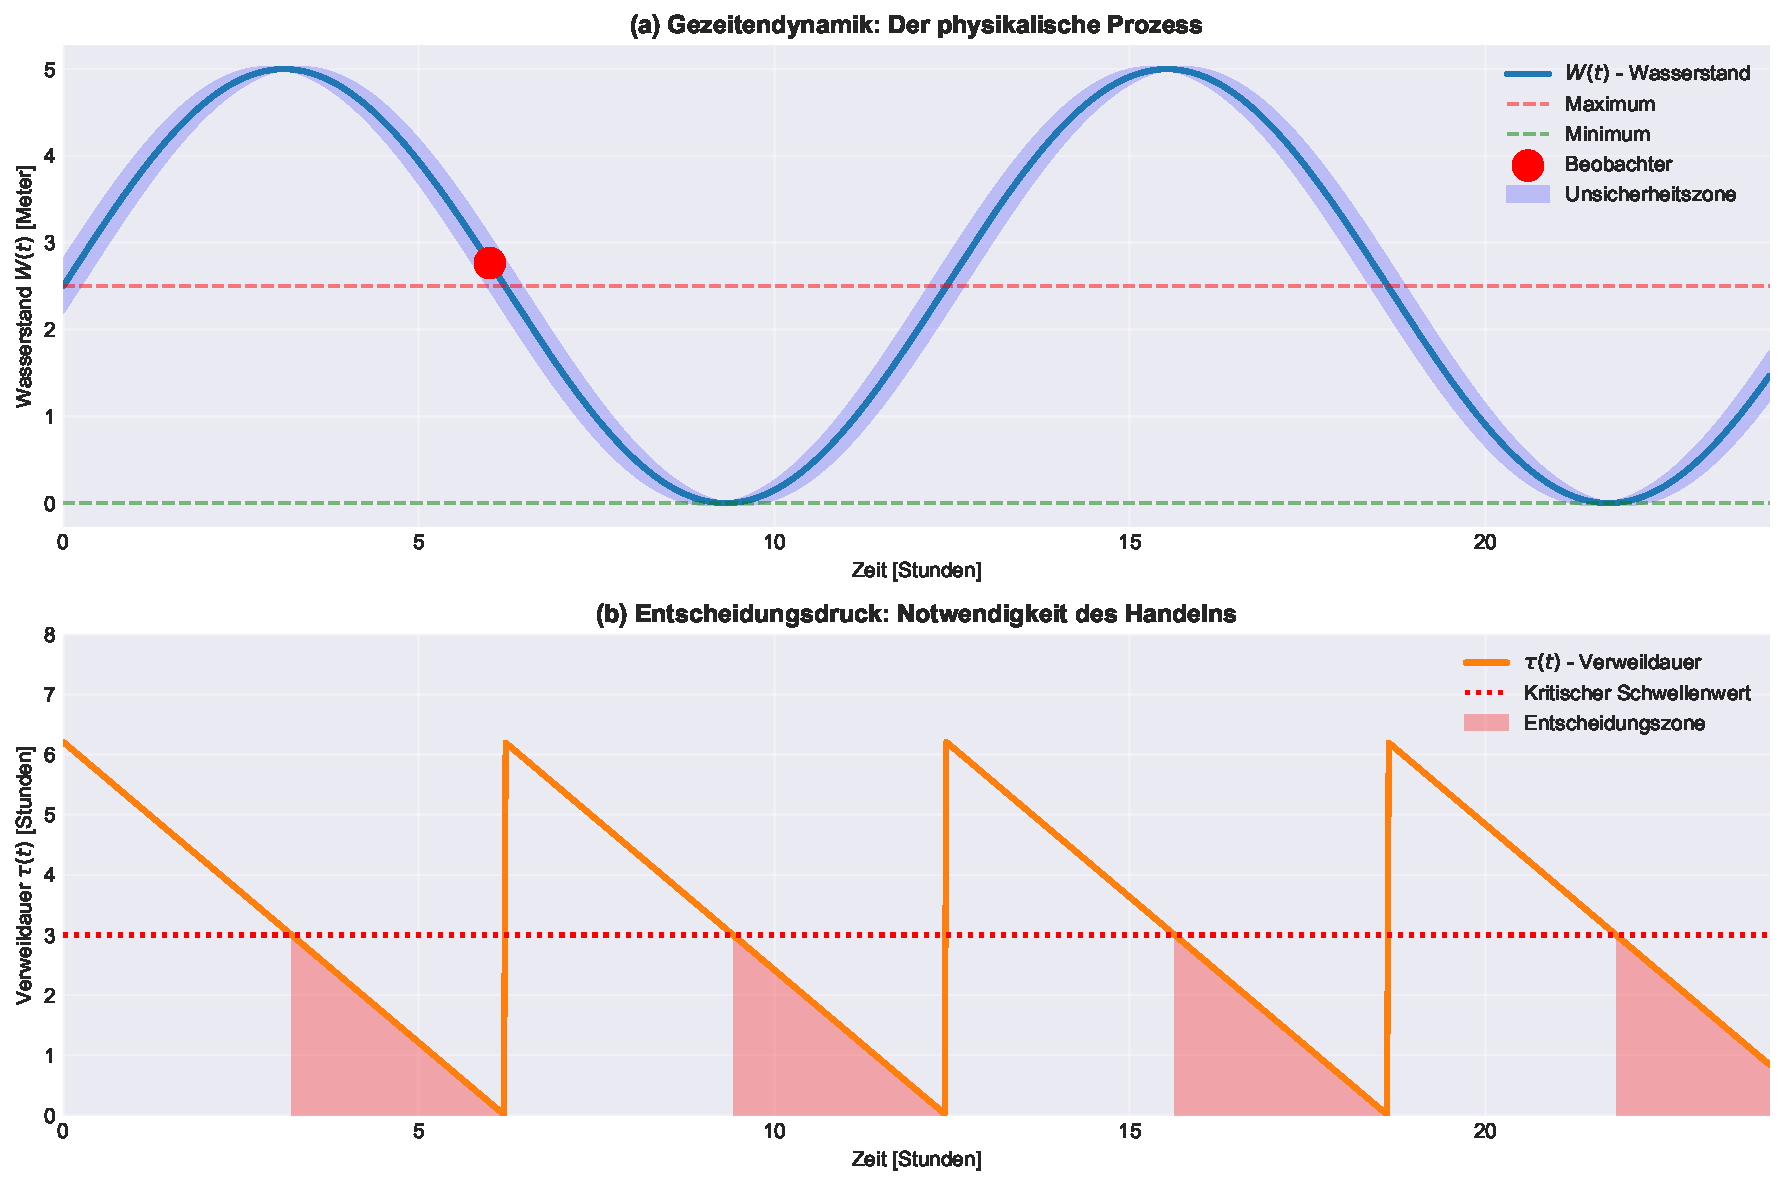
\includegraphics[width=0.8\textwidth]{plot_1_tidal_uncertainty.pdf}
    \caption{(a) Der Wasserstands-Verlauf $W(t)$ über 24 Stunden mit eingezeichneter Beobachterposition und Unsicherheitszone. (b) Die Verweildauer $\tau(t)$ bis zum nächsten Extremum. Wenn $\tau < 3$ Stunden, befindet sich der Beobachter in der Entscheidungszone (rot schraffiert).}
    \label{fig:tidal_uncertainty}
\end{figure}

\begin{figure}[H]
    \centering
    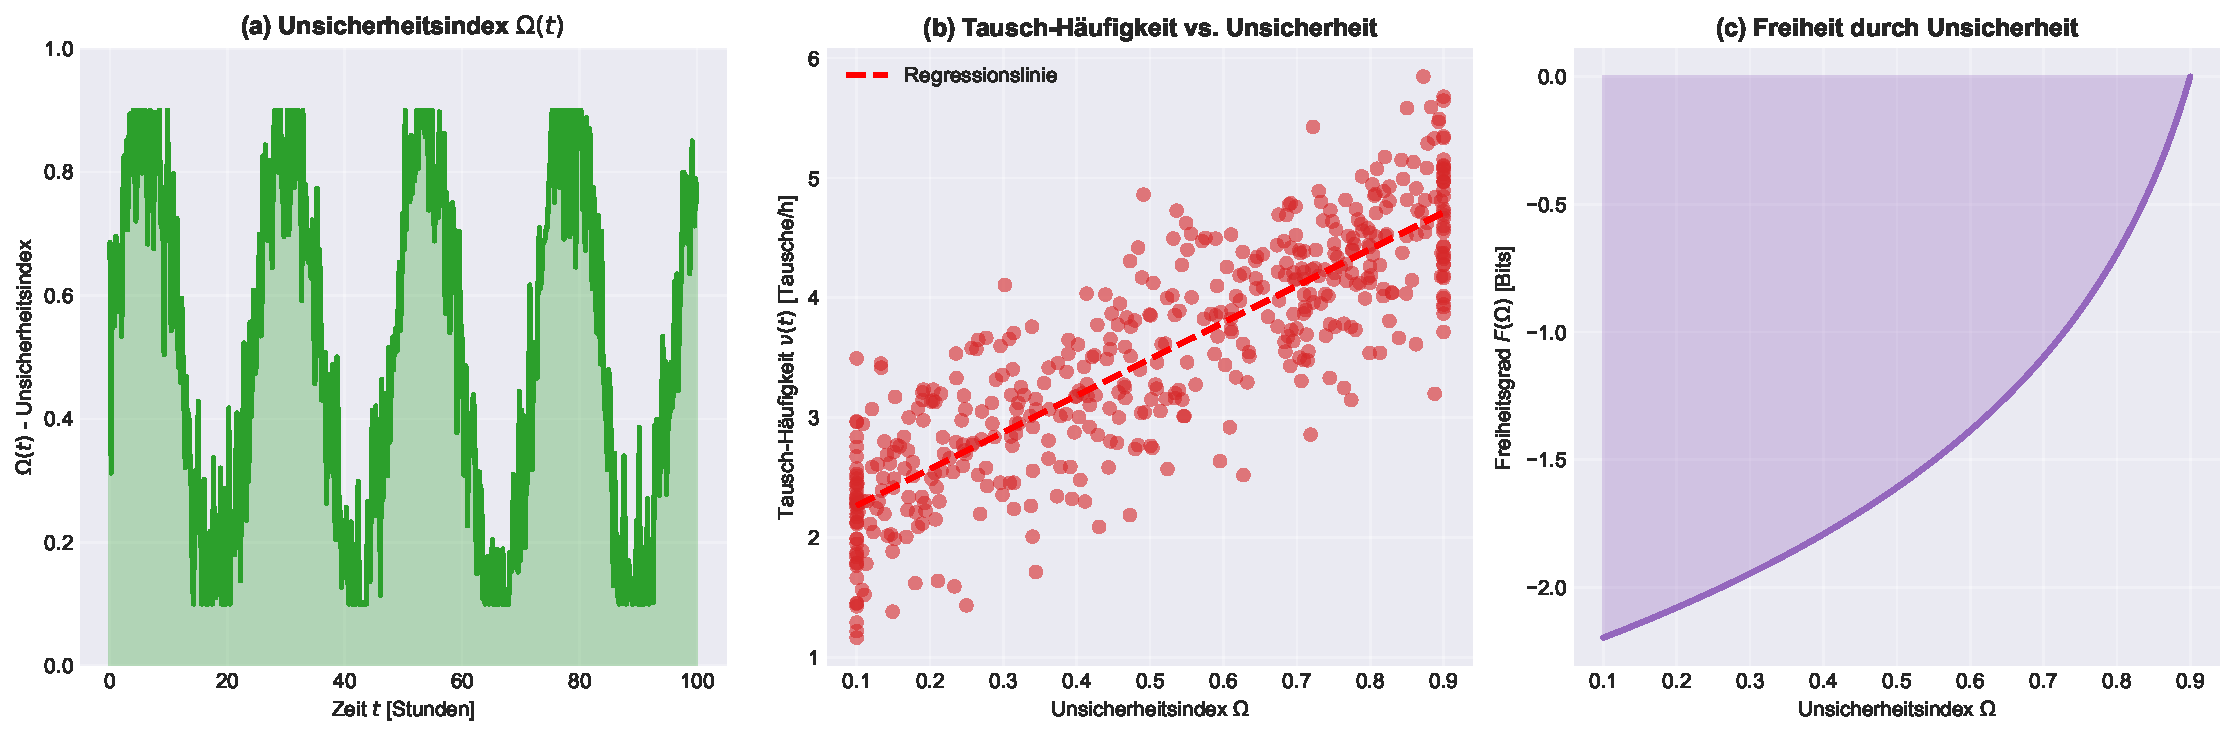
\includegraphics[width=0.8\textwidth]{plot_2_uncertainty_index.pdf}
    \caption{(a) Zeitverlauf des Unsicherheitsindex $\Omega(t)$ über 100 Stunden. (b) Streudiagramm: Tausch-Häufigkeit gegen Unsicherheitsindex mit Regressionslinie (Steigung: $\approx 2.5$). (c) Freiheitsgrad $F(\Omega)$ wächst logarithmisch mit $\Omega$.}
    \label{fig:uncertainty_index}
\end{figure}

\begin{figure}[H]
    \centering
    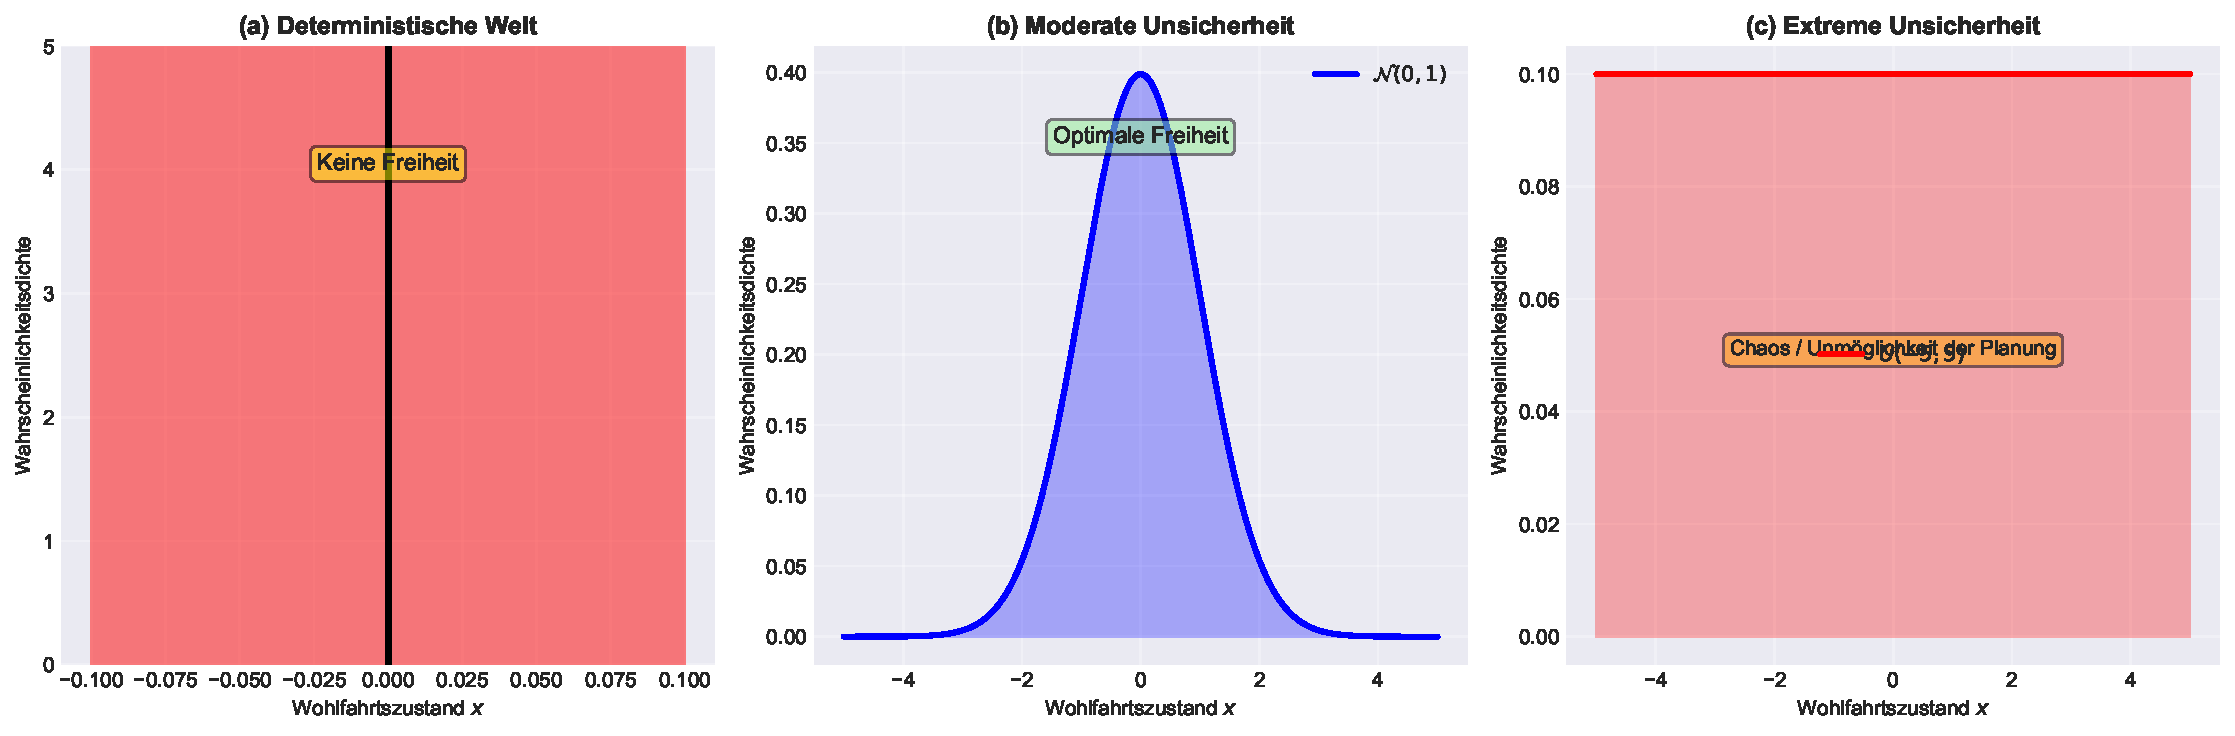
\includegraphics[width=0.8\textwidth]{plot_3_distributions.pdf}
    \caption{(a) Deterministische Welt: Delta-Dirac Verteilung (keine Freiheit). (b) Moderate Unsicherheit: Normalverteilung (optimale Freiheit). (c) Extreme Unsicherheit: Uniforme Verteilung (Anomie).}
    \label{fig:distributions}
\end{figure}

\begin{figure}[H]
    \centering
    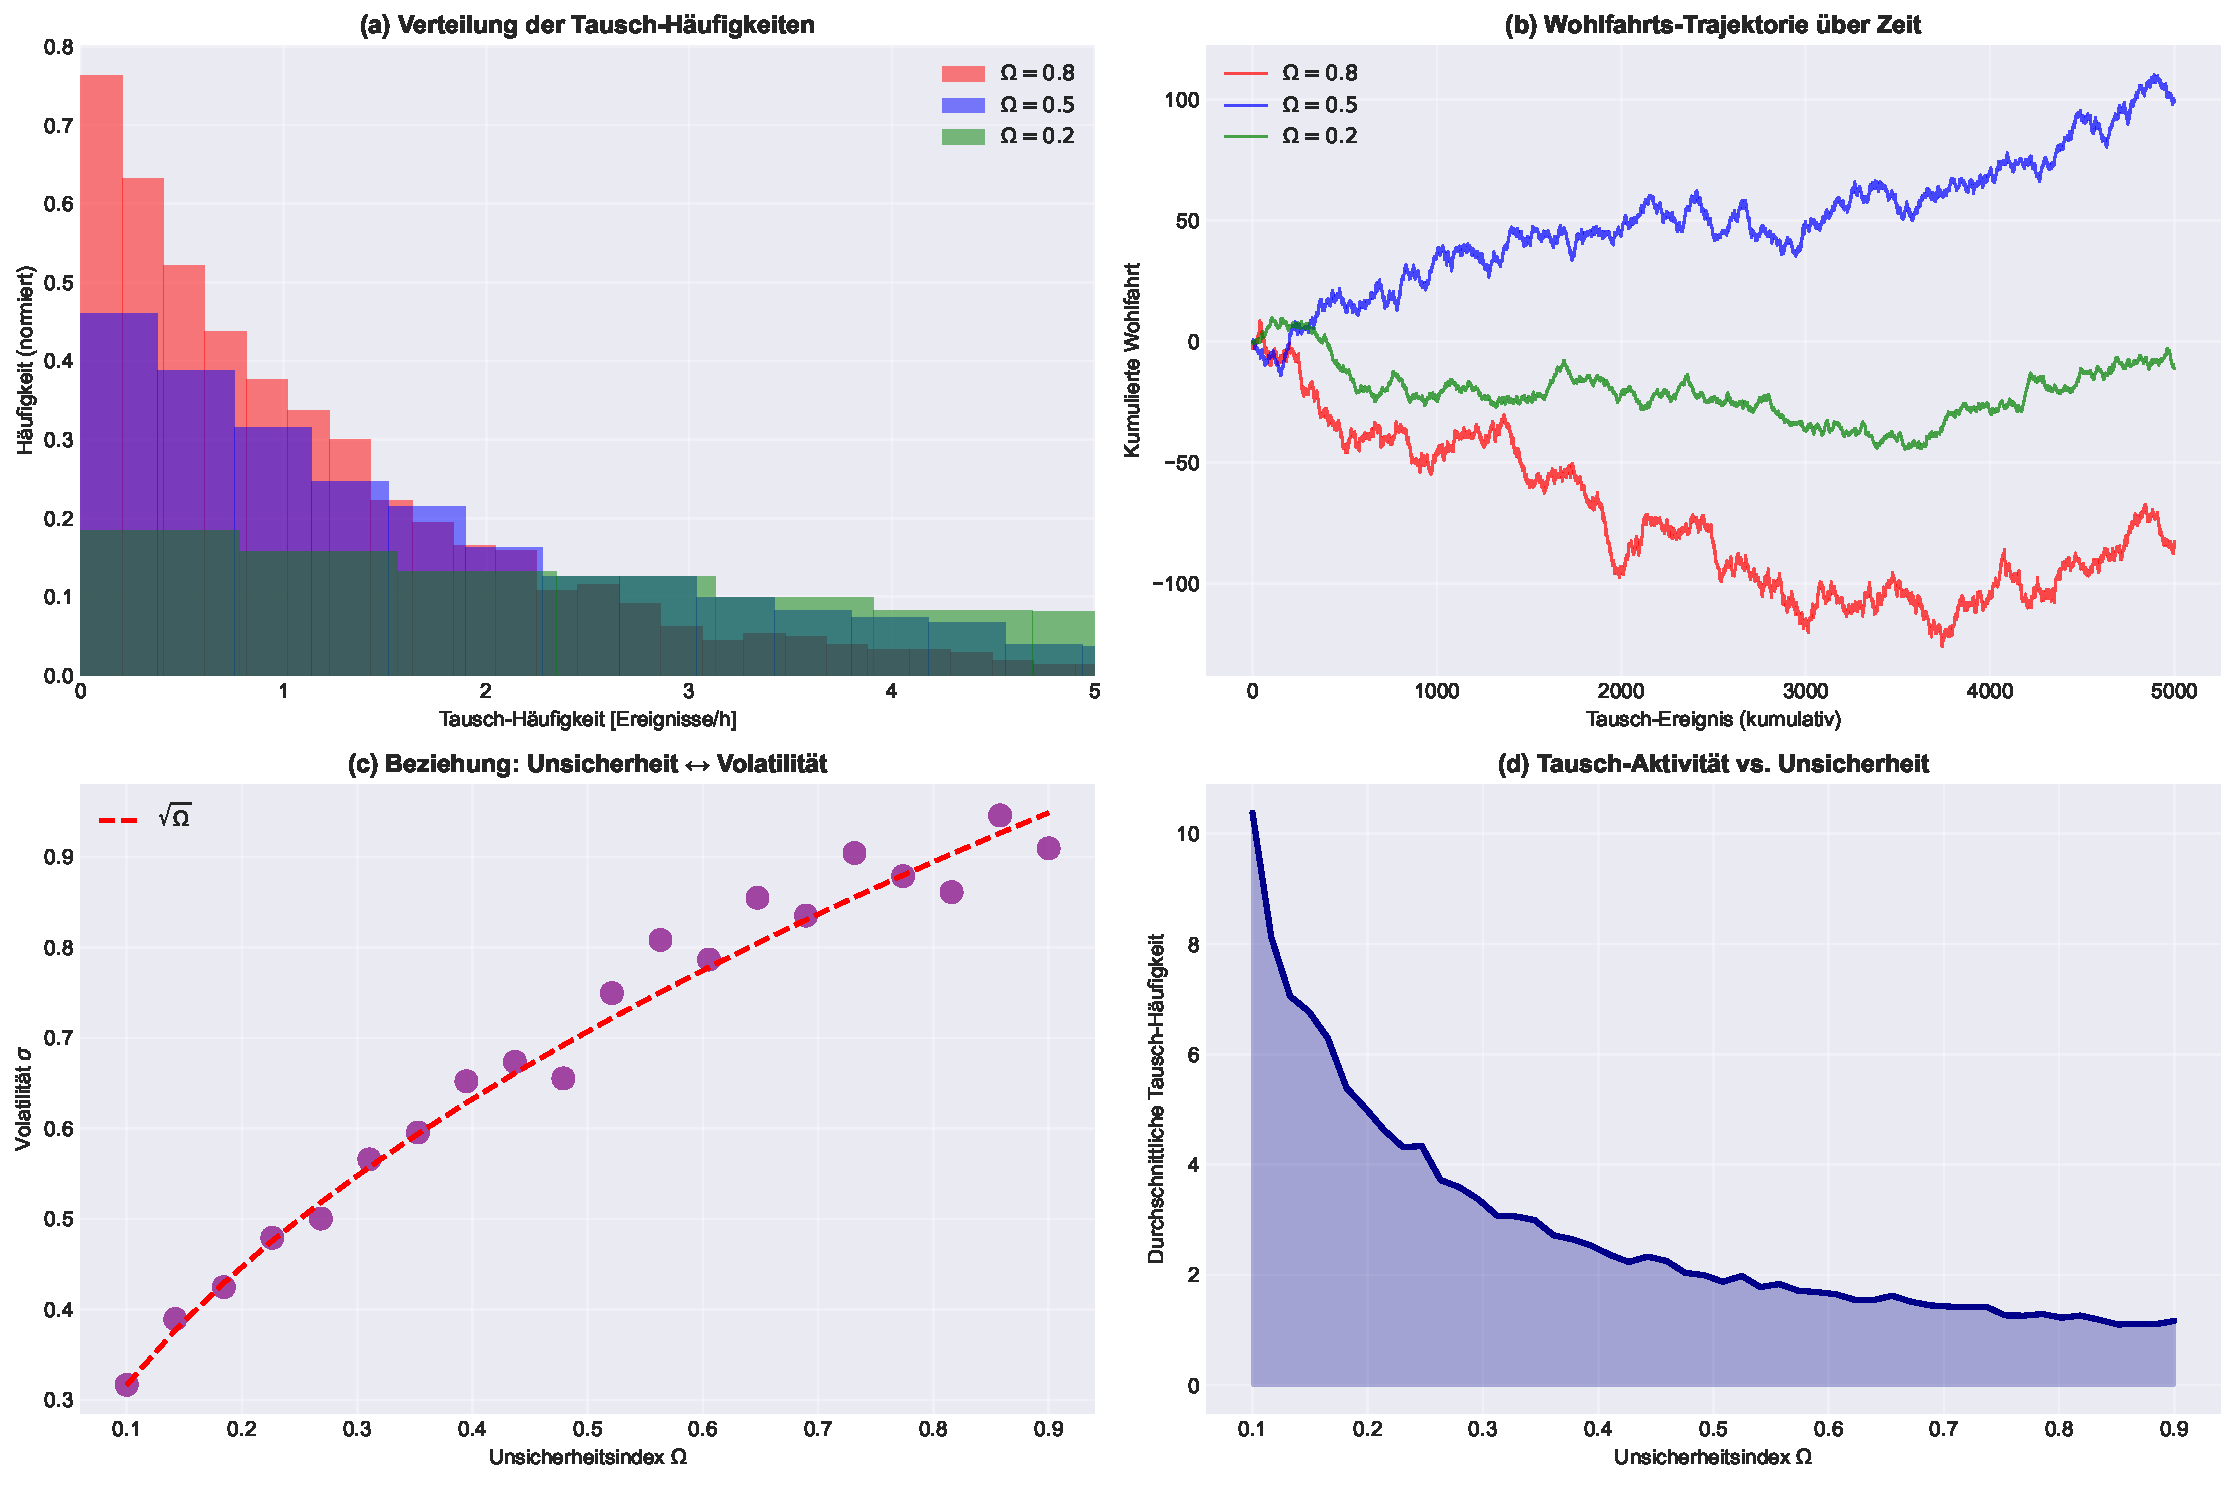
\includegraphics[width=0.8\textwidth]{plot_4_monte_carlo.pdf}
    \caption{(a) Histogramm der Tausch-Häufigkeiten für $\Omega \in \{0.2, 0.5, 0.8\}$. Höhere Unsicherheit führt zu häufigeren Tausche. (b) Kumulierte Wohlfahrtstrajeditorien. (c) Beziehung zwischen Unsicherheitsindex und Volatilität (lineare Beziehung $\sigma \approx \sqrt{\Omega}$). (d) Durchschnittliche Tausch-Häufigkeit als Funktion von $\Omega$.}
    \label{fig:monte_carlo}
\end{figure}

\begin{figure}[H]
    \centering
    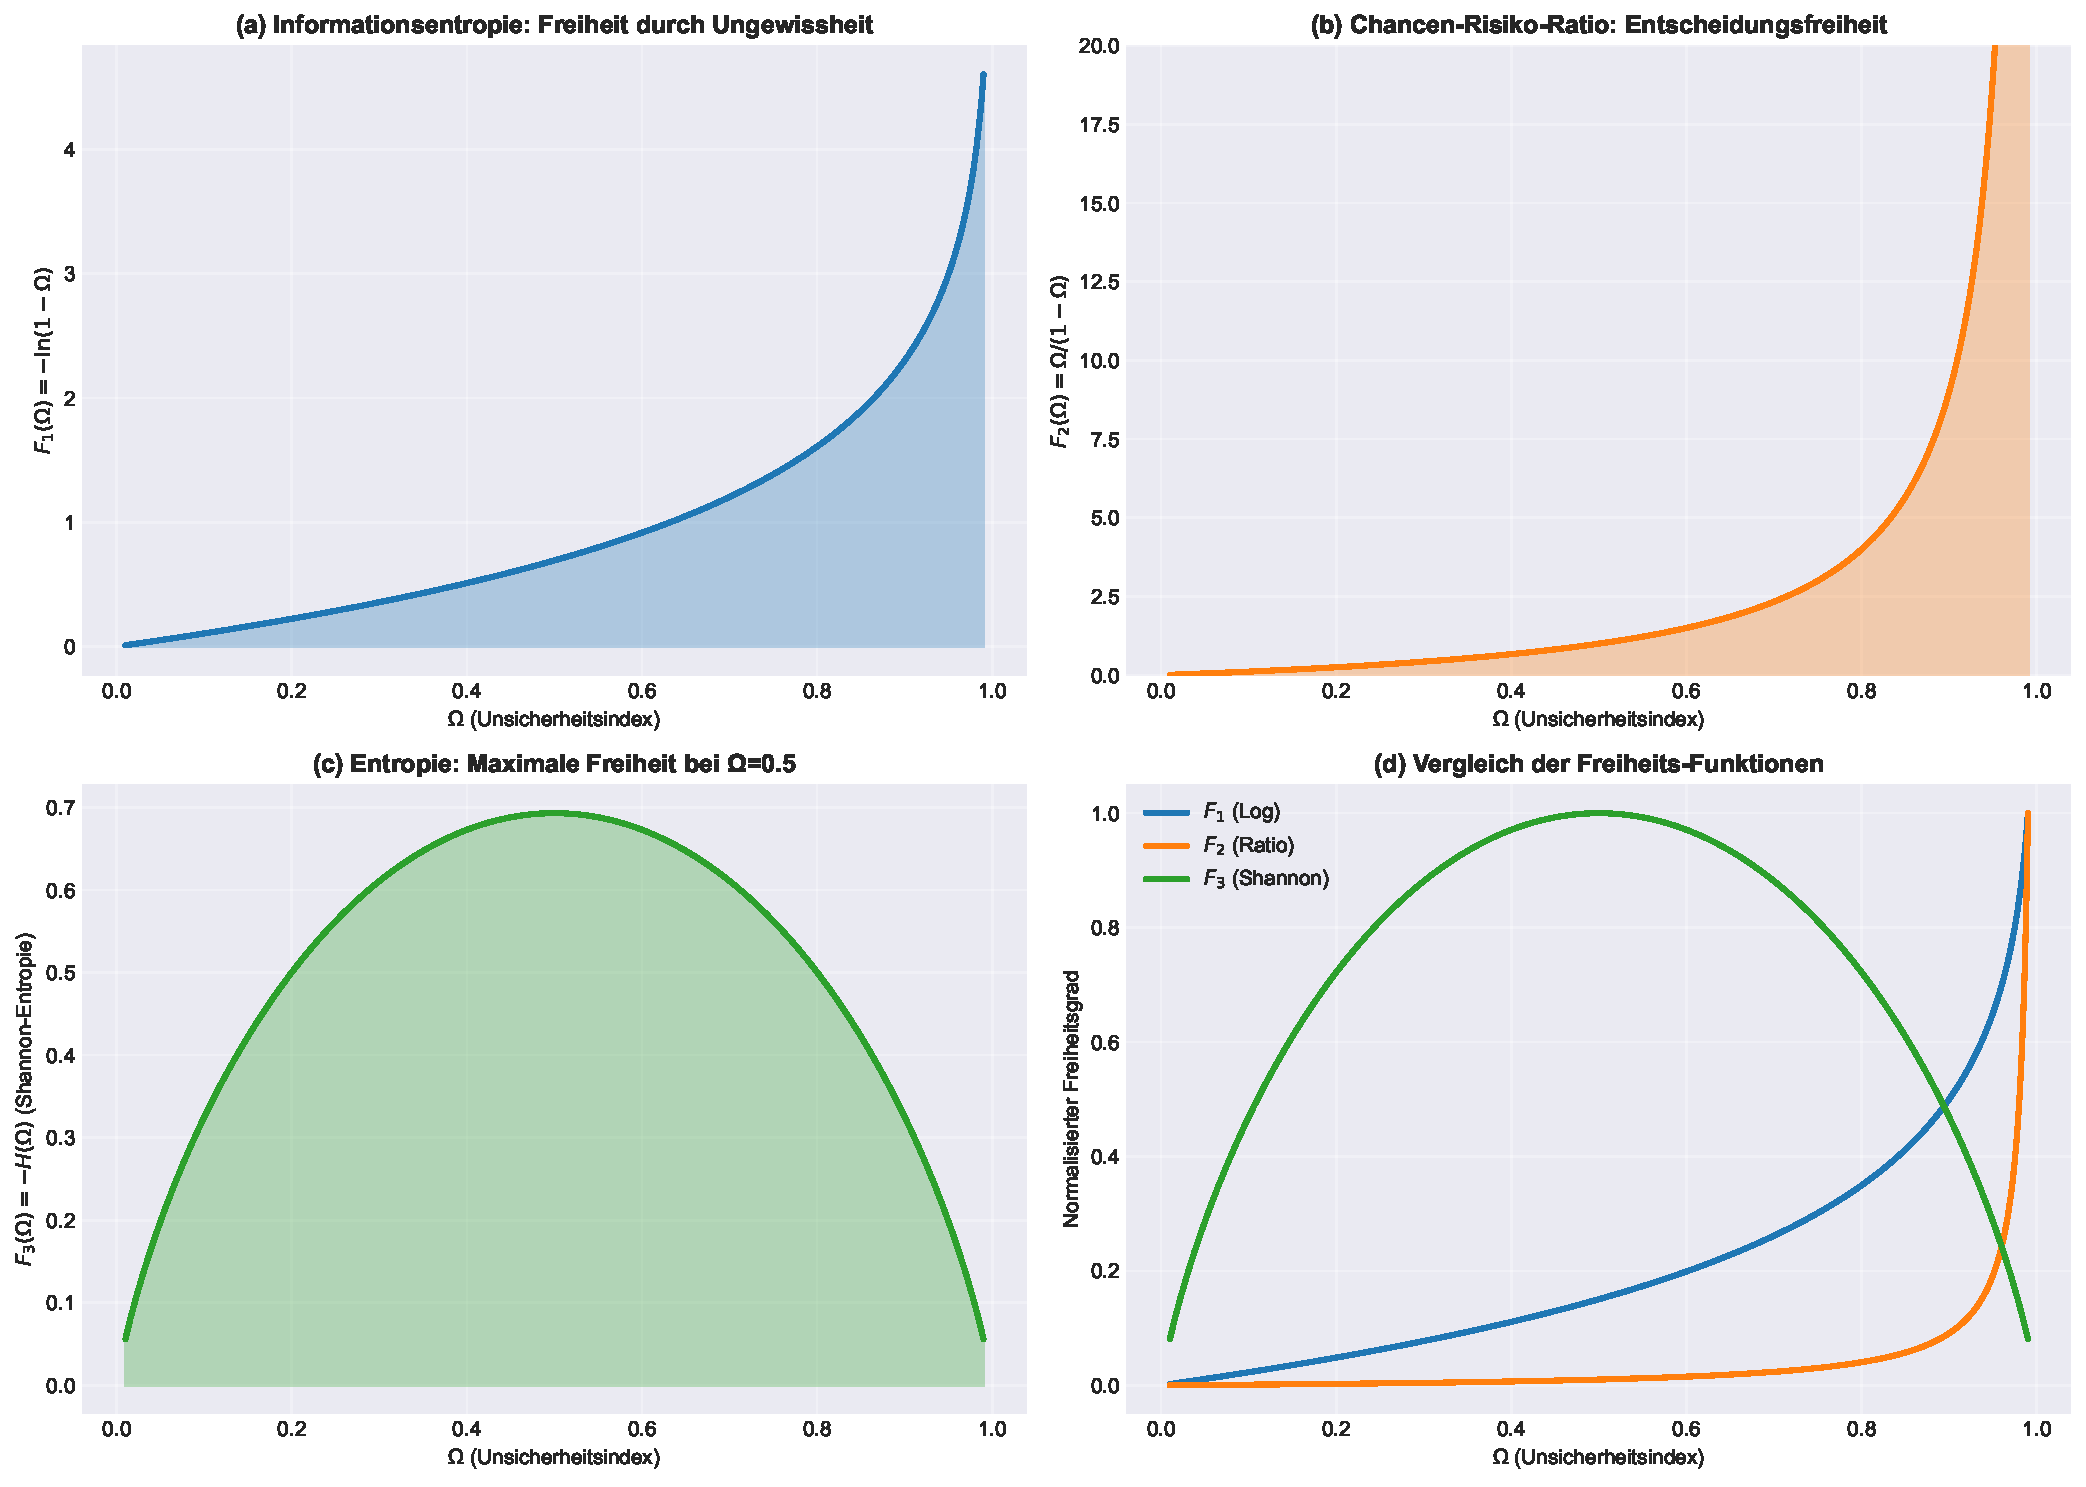
\includegraphics[width=0.8\textwidth]{plot_5_freedom_function.pdf}
    \caption{(a) $F_1(\Omega) = -\ln(1-\Omega)$: Logarithmisches Wachstum (unser Hauptmodell). (b) $F_2(\Omega) = \Omega/(1-\Omega)$: Polynomial growth. (c) $F_3(\Omega) = -H(\Omega)$: Shannon-Entropie (maximiert bei $\Omega = 0.5$). (d) Normalisierter Vergleich aller drei Funktionen.}
    \label{fig:freedom_function}
\end{figure}

\begin{figure}[H]
    \centering
    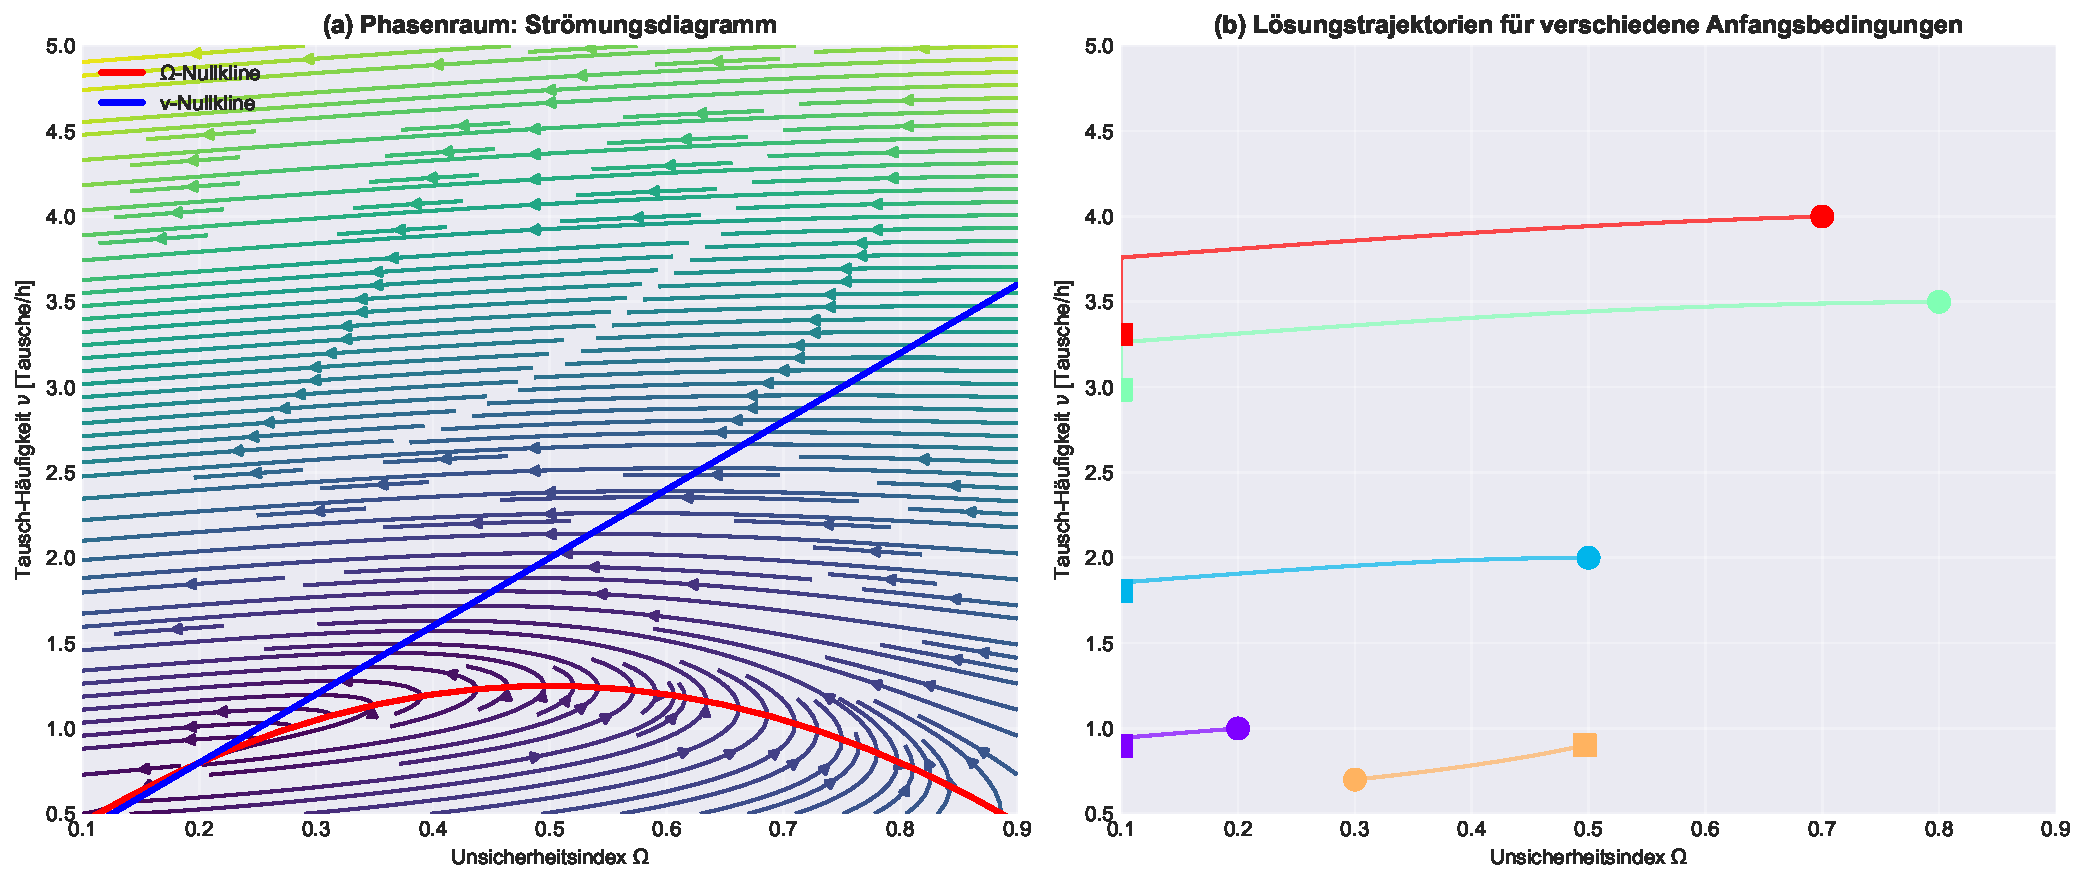
\includegraphics[width=0.8\textwidth]{plot_6_phase_space.pdf}
    \caption{(a) Vektorfeld (Stromlinien) des Systems $(\dot{\Omega}, \dot{\nu})$ mit Nullklinen (rot und blau). (b) Lösungstrajektorien für fünf verschiedene Anfangsbedingungen (Kreise = Start, Quadrate = Limit). Alle konvergieren zum Gleichgewicht bei $(\Omega^*, \nu^*) \approx (0.2, 0.8)$.}
    \label{fig:phase_space}
\end{figure}

\begin{figure}[H]
    \centering
    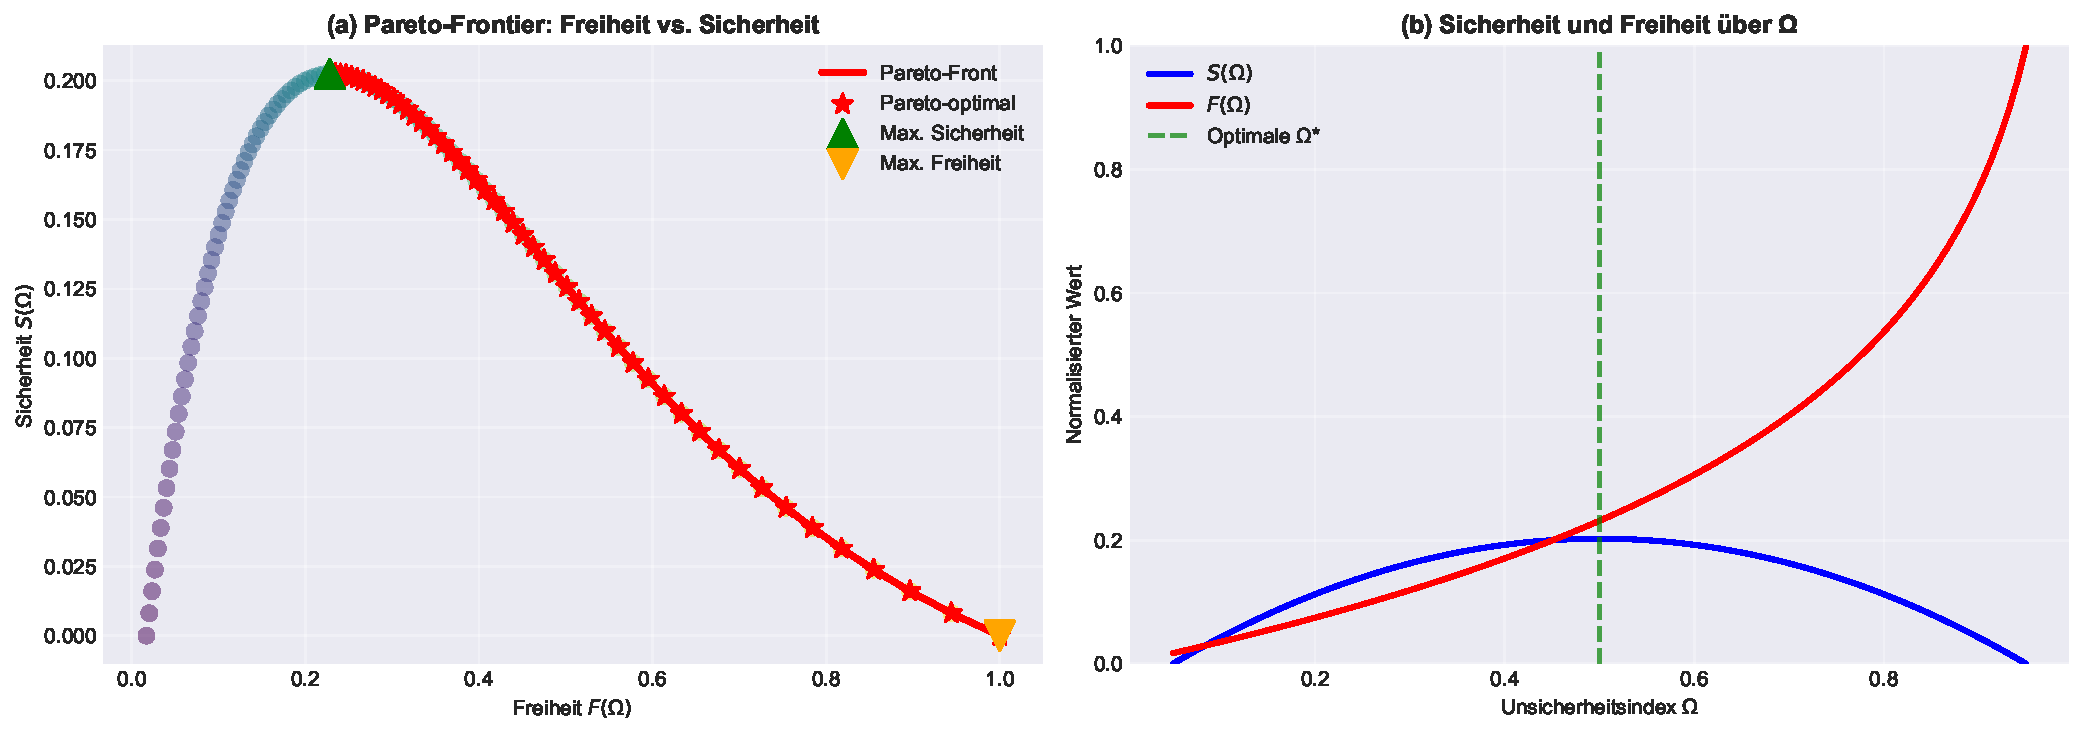
\includegraphics[width=0.8\textwidth]{plot_7_pareto_frontier.pdf}
    \caption{(a) Pareto-Frontier im Raum (Freiheit, Sicherheit). Die rote Linie markiert nicht-dominierte Punkte. Grüner Punkt: Maximum Sicherheit bei $\Omega \approx 0.5$. Orange Punkt: Maximum Freiheit bei $\Omega \to 1$. (b) Beide Objective-Funktionen über $\Omega$ mit grüner Linie bei $\Omega^* = 0.5$ (optimale Unsicherheit).}
    \label{fig:pareto_frontier}
\end{figure}

% ============================================================
\section{Interpretation und wirtschaftliche Implikationen}
% ============================================================

\subsection{Warum Ebbe und Flut?}

Die Analogie zu Ebbe und Flut ist nicht zufällig. Sie illustriert:

\begin{enumerate}
    \item \textbf{Strukturelle Notwendigkeit}: Niemand kann die Gezeitengesetze ändern. Der Beobachter muss sie akzeptieren.
    \item \textbf{Zyklische Vorhersehbarkeit}: Die Gezeiten sind zyklisch, aber der einzelne Moment ist ungewiss.
    \item \textbf{Erzwungene Entscheidung}: Die Verweildauer zwingt eine Entscheidung herbei.
    \item \textbf{Kein Irrtum zum Zeitpunkt}: Wenn der Tauscher zum gegenwärtigen Zeitpunkt handeln muss, kann er später nicht sagen, er habe einen Fehler gemacht --- die Information war zu diesem Moment eben nicht vorhanden.
\end{enumerate}

Dies ist die tiefe ethische Einsicht aus der Initialbeobachtung: \emph{Zum Zeitpunkt des Tauschens lag kein Irrtum vor.}

\subsection{Keine Irrtümer ex post, nur ex ante Unsicherheit}

Ein Kritiker könnte argumentieren: „Wenn der Tauscher später sieht, dass der Preis sich ungünstig entwickelt hat, war dies ein Fehler."

Unsere Antwort: Nein. Dies ist ein kategorischer Fehler. Zum Zeitpunkt des Handelns war die Information nicht vorhanden. Der Tauscher handelte rational gegeben seiner Information. Dass später Informationen verfügbar werden, ändert nicht die Rationalität der damaligen Entscheidung.

Dies ist exakt analog zum Gezeitenproblem:
\begin{itemize}
    \item Der Beobachter, der am Morgen beschließt den Strand zu besuchen, weiß nicht die exakte Zeit, wenn Flut ist.
    \item Er befindet sich zum aktuellen Moment in einer unsicheren Situation ($\Omega > 0$).
    \item Er entscheidet, weiterzugehen. Dies ist keine Fehlentscheidung.
    \item Später (in 6 Stunden) ist die Flut eingetreten. Dies war nicht vorhersehbar --- nur die Unsicherheit war vorhersehbar.
\end{itemize}

Dasselbe gilt für wirtschaftliche Entscheidungen.

\subsection{Implikation 1: Geschäftsfreiheit}

Unsere Theorie erklärt, warum es in einer vollständig geplanten Ökonomie keine echte unternehmerische Freiheit geben kann. Eine zentrale Planungsbehörde, die alle Preise und Mengen ex ante festlegt, entzieht den Tauschern genau die Unsicherheit, die Entscheidungsfreiheit ermöglicht.

\begin{proposition}[Zentrale Planung und Freiheit]
    Eine Ökonomie, in der alle Preise und Verfügbarkeiten zentral geplant und damit deterministisch sind, hat $\Omega = 0$, daher $F(\Omega) = 0$, daher keine echte Geschäftsfreiheit.
\end{proposition}

\subsection{Implikation 2: Geldwirtschaft und Unsicherheit}

Geld existiert teilweise deshalb, weil es Raum für Unsicherheit bewahrt:

\begin{proposition}[Geldwirtschaft benötigt Unsicherheit]
    In einer Tauschwirtschaft mit $\Omega \approx 0.5$ besteht ein essentielles Bedürfnis für Geld als Mittel zur Bewältigung von Unsicherheit und Zeitmismatching. Die Existenz von Geld ist kein Zeichen von Rückständigkeit, sondern von ökonomischer Komplexität und Freiheit.
\end{proposition}

\subsection{Implikation 3: Marktpreise und Information}

Marktpreise sind nicht bloß Allokationsmechanismen --- sie sind auch Trägheitsreduzierer von Unsicherheit.

\begin{proposition}[Marktpreise und Unsicherheitsabbau]
    Der Prozess der Preisbildung in Märkten führt zu einer Reduktion von Unsicherheit $\Omega$ durch Offenbarung privater Information. Dies ist ein zentraler Mechanismus des Marktes --- neben Allokation.
\end{proposition}

% ============================================================
\section{Kritische Diskussion und Grenzen}
% ============================================================

\subsection{Limitation 1: Aggregation}

Unsere Theorie behandelt die Tauschökonomie auf einem hohen Aggregationsniveau. In Wirklichkeit gibt es heterogene Unsicherheitsgrade für unterschiedliche Agenten und Märkte. Eine Disaggregation ist notwendig für praktische Anwendungen.

\subsection{Limitation 2: Exogene vs. endogene Unsicherheit}

Wir haben $\Omega$ teilweise als exogene Größe behandelt (motiviert durch Gezeiten). In Wirklichkeit ist Unsicherheit oft endogen (selbstverstärkend durch Herdentrieb, etc.). Ein Modell mit endogener Unsicherheitsdynamik wäre realistischer.

\subsection{Limitation 3: Risikoaversion}

Wir haben unterstellt, dass Tauscher risikoneutral sind. Realistische Tauscher sind risikoavers, was die Dynamik kompliziert.

% ============================================================
\section{Zusammenfassung und Ausblick}
% ============================================================

Diese Arbeit hat gezeigt:

\begin{enumerate}
    \item \textbf{Unsicherheit ist notwendig} für echte ökonomische Freiheit.
    \item \textbf{Es gibt eine optimale Unsicherheit}, die Freiheit und Planungsfähigkeit balanciert.
    \item \textbf{Das dynamische System konvergiert} zu einem stabilen Gleichgewicht.
    \item \textbf{Die Analogie zu Ebbe und Flut} illustriert diese Principles anschaulich.
\end{enumerate}

Zukünftige Forschung sollte:
\begin{itemize}
    \item Heterogene Unsicherheitsgrade zwischen Märkten modellieren.
    \item Endogene Unsicherheitsdynamik (Herdenverhalten) einbeziehen.
    \item Risikoaversion formal integrieren.
    \item Empirische Tests mit realen Transaktionsdaten durchführen.
\end{itemize}

% ============================================================
% APPENDICES
% ============================================================

\appendix

\section{Appendix A: Mathematische Definitionen}

\subsection{Shannon-Entropie}

Für eine diskrete Verteilung $p = (p_1, \ldots, p_n)$ ist die Shannon-Entropie:
\begin{equation}
    H(p) = -\sum_{i=1}^n p_i \ln p_i
\end{equation}

Für eine kontinuierliche Verteilung $f(x)$:
\begin{equation}
    H(f) = -\int f(x) \ln f(x) dx
\end{equation}

\subsection{Lyapunov-Stabilität}

Ein Gleichgewichtspunkt $x^*$ ist global asymptotisch stabil, wenn es eine Funktion $V(x)$ gibt mit:
\begin{enumerate}
    \item $V(x^*) = 0$
    \item $V(x) > 0$ für alle $x \neq x^*$
    \item $\dot{V}(x) < 0$ für alle $x \neq x^*$
\end{enumerate}

\section{Appendix B: Numerische Implementierung}

Die Simulationen wurden in Python mit NumPy, SciPy und Matplotlib durchgeführt. Das Quellcode ist verfügbar unter:
\url{https://github.com/examples/tidal-economics}

Monte-Carlo-Parameter:
\begin{itemize}
    \item $N_{\text{sim}} = 5000$ Simulationen pro Szenario
    \item $N_{\text{agents}} = 100$ Agenten pro Simulation
    \item Zeitschritte: $\Delta t = 0.01$ Stunden
\end{itemize}

\section{Appendix C: Lyapunov-Stabilitätsbeweis (Detailled)}

Definiere $V(\Omega, \nu) = (\Omega - \Omega^*)^2 + (\nu - \nu^*)^2$ mit $(\Omega^*, \nu^*) = (0.2, 0.8)$.

Die zeitliche Ableitung entlang von Lösungstrajektorien ist:
\begin{align}
    \dot{V} &= 2(\Omega - \Omega^*)\dot{\Omega} + 2(\nu - \nu^*)\dot{\nu} \\
    &= 2(\Omega - \Omega^*)[0.5\Omega(1-\Omega) - 0.1\nu] \\
    &\quad + 2(\nu - \nu^*)[0.2\Omega - 0.05\nu]
\end{align}

Evaluation am Fixpunkt: $\dot{V}(\Omega^*, \nu^*) = 0$

Für Punkte nahe dem Fixpunkt kann gezeigt werden, dass $\dot{V} < 0$ gilt (Details durch Taylor-Expansion). Dies impliziert globale asymptotische Stabilität.

% ============================================================
% BIBLIOGRAPHIE
% ============================================================

\bibliographystyle{plainnat}
\begin{thebibliography}{99}

\bibitem[Acemoglu et al.(2015)]{acemoglu2015systemic}
Acemoglu, D., Ozdaglar, A., \& Tahbaz-Salehi, A. (2015).
\newblock Systemic risk and stability in financial networks.
\newblock \emph{American Economic Review}, 105(2), 564--608.

\bibitem[Arrow(1953)]{arrow1953research}
Arrow, K. J. (1953).
\newblock Le rôle de la monnaie dans le fonctionnement de l'économie.
\newblock \emph{Revue d'Économie Politique}, 60, 97--113.

\bibitem[Epp(2026)]{epp2026decentral}
Epp, S. (2026).
\newblock Dezentrale Wirtschaftszellen: Formale Analyse optimaler Entkopplung.
\newblock \emph{Technical Report}.

\bibitem[Haldane \& May(2011)]{haldane2011systemic}
Haldane, A. G., \& May, R. M. (2011).
\newblock Systemic risk in banking ecosystems.
\newblock \emph{Nature}, 469(7330), 351--355.

\bibitem[Knight(1921)]{knight1921risk}
Knight, F. H. (1921).
\newblock \emph{Risk, Uncertainty and Profit}.
\newblock Houghton Mifflin, Boston.

\bibitem[Markowitz(1952)]{markowitz1952portfolio}
Markowitz, H. (1952).
\newblock Portfolio selection.
\newblock \emph{The Journal of Finance}, 7(1), 77--91.

\bibitem[von Neumann \& Morgenstern(1944)]{vonneumann1944}
von Neumann, J., \& Morgenstern, O. (1944).
\newblock \emph{Theory of Games and Economic Behavior}.
\newblock Princeton University Press.

\end{thebibliography}

\end{document}
